\documentclass[conference]{IEEEtran}
\IEEEoverridecommandlockouts
\usepackage{cite}
\usepackage{amsmath,amssymb,amsfonts}
\usepackage{algorithmic}
\usepackage{graphicx}
\usepackage{textcomp}
\usepackage{xcolor}
\usepackage{tikz}
\usetikzlibrary{arrows.meta,positioning,fit,backgrounds,shapes.geometric}
\def\BibTeX{{\rm B\kern-.05em{\sc i\kern-.025em b}\kern-.08em
    T\kern-.1667em\lower.7ex\hbox{E}\kern-.125emX}}
\begin{document}

\title{Quality-Adaptive Loss Reweighting Using Expert-Assigned Image Quality for Robust Skin Lesion Classification}

\author{
\IEEEauthorblockN{1\textsuperscript{st} Given Name Surname}
\IEEEauthorblockA{\textit{Department Name} \\
\textit{Institution Name}\\
City, Country \\
email@example.com}
}

\maketitle

\begin{abstract}
Diagnostic image quality varies widely in clinical practice, yet quality-aware training methods have had to estimate quality from image statistics or feature norms rather than observe it, because expert judgments of image quality are almost never recorded alongside diagnostic labels. This paper has proposed quality-adaptive loss reweighting, which scales each training sample's classification loss by a real expert-assigned rating of its diagnostic image. Two opposing directions have been evaluated: down-weighting low-quality samples as less reliable, and up-weighting them to force the model to learn from difficult images. The second, the opposite of what the closest face recognition precedents apply, has improved balanced accuracy by 0.037 and malignant sensitivity by 0.092 over an identical baseline. Because a gain of this size is comparable to the fold-to-fold standard deviation, we have validated it causally rather than statistically: a permutation test, preserving the weight distribution but permuting the lesion-to-rating assignment, has returned performance to baseline, with the real result lying above every permutation drawn, establishing that the improvement has depended on the quality signal's information content rather than on generic reweighting. The full pipeline has reached 0.840 balanced accuracy, of which 65\% of the total gain has been attributable to the quality-adaptive loss and the remainder to generic evaluation-time averaging. The method has been made possible by MCR-SL, the only public skin lesion dataset recording per-image expert quality ratings, on which we have also reported the first published benchmark and six robustness analyses, three of which have reversed an apparent positive result.
\end{abstract}

\begin{IEEEkeywords}
skin lesion classification, multimodal fusion, dermoscopy, image quality, metadata fusion, deep learning, medical imaging benchmark
\end{IEEEkeywords}

\section{Introduction}
Medical images acquired in routine practice vary substantially in diagnostic quality. Lighting, focus, framing, and hair occlusion all degrade the evidence a classifier receives, and training as though every image were equally informative assumes a uniformity clinical data does not have. Face recognition has addressed this by making the objective quality aware: AdaFace \cite{adaface} and MagFace \cite{magface} adapt each sample's margin from an estimate of image quality derived from the feature norm, both reducing emphasis on difficult low-quality samples. That reliance on an estimated proxy is a necessity, not a preference, because face datasets do not record what an expert thought of each photograph.

Skin lesion classification has followed a parallel path. Convolutional networks have reached dermatologist-level accuracy on large single-modality archives \cite{esteva2017,ham10000}, and a smaller line of work has fused images with patient metadata \cite{metablock,paduf20}. In neither case has a per-image expert judgment of quality been available, so quality has remained something to be inferred rather than observed.

MCR-SL \cite{mcrsl} has removed that constraint, and is the reason the method proposed here is possible at all. It has paired 779 clinical and 1352 dermoscopic images across 240 lesions from 60 subjects with twenty-two subject-level metadata fields and, distinctively, with a one-to-ten quality rating that dermatologists have assigned to the specific image used for each lesion's diagnosis. It is, to our knowledge, the only public skin lesion dataset carrying such a field, which makes it the enabling dataset for a loss function driven by real expert quality rather than an estimated proxy, not merely a convenient testbed for a pre-existing method.

This paper has therefore asked two separable questions: whether performance degrades on lower-quality images, and whether the training objective can use the quality signal to improve robustness. The answers have differed, the first a null result and the second a positive one validated by a causal control.

\subsection{Contributions}
This paper has made the following contributions.
\begin{itemize}
\item \textbf{Quality-adaptive loss reweighting:} a scheme that scales each sample's classification loss by a real expert-assigned image-quality rating. The direction that has worked, up-weighting low-quality samples, is the opposite of the face recognition precedents that motivated it, and we have offered a domain-specific explanation for why.
\item \textbf{Causal validation via a shuffled-quality control:} permuting the lesion-to-rating assignment while preserving the weight distribution has removed the entire gain, establishing that it has depended on the quality signal's information content and not on generic per-sample reweighting.
\item \textbf{A first published benchmark on MCR-SL:} evaluated under a subject-disjoint stratified five-fold protocol, together with a sweep of eleven follow-up configurations that has isolated which interventions help at this scale and which do not.
\item \textbf{Six robustness analyses, including three reversed findings:} enabled by MCR-SL's quality ratings and partial histopathology confirmation, and reported together with the three cases in which an apparent positive finding has not survived a control.
\end{itemize}

\subsection{Research Gap}
To the authors' knowledge, no prior work has used a direct expert rating of image quality as a loss-reweighting signal in medical image classification. Quality-aware objectives have relied on estimated proxies, quality-aware medical methods have acted on the architecture rather than the loss, and the closest loss-weighting scheme on skin lesions derives its difficulty signal from the model rather than from a human judgment of the photograph. Section~\ref{sec:lit} substantiates each of these in turn.

\section{Literature Review}
\label{sec:lit}
Image-only dermoscopic classification has been studied extensively since Esteva \emph{et al.} \cite{esteva2017} matched dermatologist performance on a curated archive, with HAM10000 \cite{ham10000} becoming a standard benchmark. These studies have treated the image as the sole input.

Metadata fusion is a distinct thread. Pacheco and Krohling \cite{metablock} have proposed the Metadata Processing Block, which reweights image features using patient metadata, evaluated on PAD-UFES-20 \cite{paduf20} (2298 clinical images, 1641 lesions). That dataset is the closest comparator in problem shape and is our primary external reference point (Section~\ref{sec:comparison}).

Quality-aware training has been developed most fully in face recognition. AdaFace \cite{adaface} adapts the angular margin using the feature norm as a quality proxy, reducing emphasis on hard examples when an image is estimated to be low quality, since a degraded and difficult face is likely unidentifiable and forcing separation would fit noise. MagFace \cite{magface} ties feature magnitude to quality similarly. Both depend on an estimated proxy rather than a recorded human judgment.

Within medical imaging, quality has more often been handled architecturally. QGDR \cite{qgdr} routes fundus images through quality-conditioned expert branches for diabetic retinopathy grading, modifying the architecture rather than the loss, and derives its quality states largely from predicted pseudo-labels rather than from expert annotation.

Closest to this work, Hu and Yang \cite{hu2023} have applied knowledge-based loss weighting on HAM10000, assigning weights at the class level, favouring minority classes, and at the instance level, favouring challenging samples. Their instance-level term shares this paper's direction in emphasising difficult examples, but its notion of difficulty is derived from the model and data themselves. The signal used here is external to both: an expert's judgment of the photograph, recorded independently of how any model performs on it. Our fusion module draws on Squeeze-and-Excitation \cite{se} and is used as an established component, not claimed as a contribution.

\section{Proposed Methodology}
Fig.~\ref{fig:arch} summarizes the architecture. This paper has proposed a channel-gated fusion method for cross-modal skin lesion classification and has compared it against two baselines under an identical training and evaluation protocol.

\subsection{Architecture}
\label{sec:arch}
Fig.~\ref{fig:arch} shows the pipeline left to right, and this subsection follows it in that order. On the upper path, an ImageNet-pretrained EfficientNet-B0 \cite{efficientnet,imagenet} encodes the dermoscopic image, returning both a 1280-dimensional pooled vector and the final convolutional feature map. On the lower path, a metadata encoder embeds sixteen categorical fields (twelve dimensions each, with a reserved index for missing values, which are never imputed) and four numeric fields (z-scored on training-fold statistics only, each paired with a missingness indicator), and passes their concatenation through a two-layer perceptron to a 128-dimensional vector.

Two fusion variants share a common 256-dimensional projection. The late-fusion baseline concatenates the pooled image and metadata vectors. The channel-gated variant, where the two paths meet at $\otimes$ in Fig.~\ref{fig:arch}, maps the metadata vector through a linear layer and sigmoid to a 1280-dimensional gate, multiplies the feature map channel by channel, and then pools. This is the Squeeze-and-Excitation mechanism \cite{se} conditioned on metadata rather than on the feature map itself, and is used here as an established component rather than claimed as a contribution of this paper. A binary head and a nine-class auxiliary head sit on the fused vector; a third head predicting the quality rating is added only for the quality-aware variant reported as a negative result below.


\begin{figure}[htbp]
\centering
\resizebox{\linewidth}{!}{%
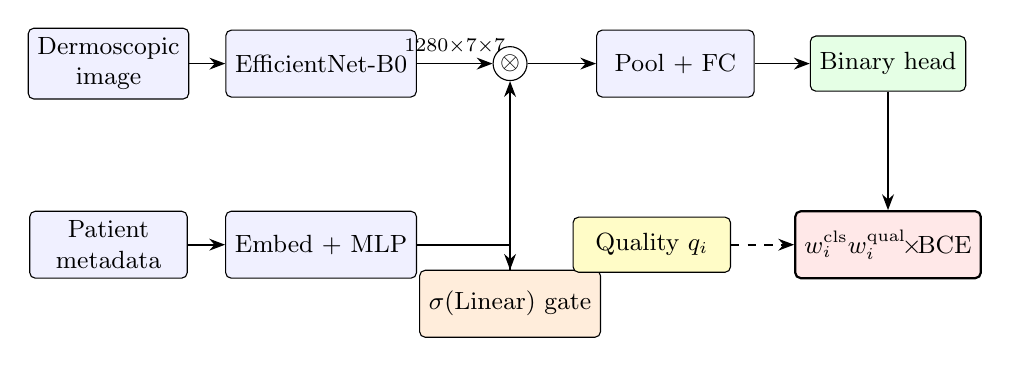
\begin{tikzpicture}[
  box/.style={draw, rounded corners=2pt, align=center, minimum height=0.85cm, minimum width=2.0cm, font=\small, fill=blue!6},
  gbox/.style={draw, rounded corners=2pt, align=center, minimum height=0.85cm, minimum width=2.0cm, font=\small, fill=orange!14},
  hbox/.style={draw, rounded corners=2pt, align=center, minimum height=0.7cm, minimum width=1.7cm, font=\small, fill=green!10},
  lbox/.style={draw, rounded corners=2pt, align=center, minimum height=0.85cm, minimum width=2.1cm, font=\small, fill=red!9, thick},
  qbox/.style={draw, rounded corners=2pt, align=center, minimum height=0.7cm, minimum width=2.0cm, font=\small, fill=yellow!22},
  opn/.style={draw, circle, font=\small, inner sep=1pt},
  arr/.style={-Stealth, semithick}
]
% image path (top), left to right
\node[box] (img) at (0,1.15)  {Dermoscopic\\image};
\node[box] (enc) at (2.7,1.15){EfficientNet-B0};
\node[opn] (mul) at (5.1,1.15){$\otimes$};
\node[box] (pool)at (7.2,1.15){Pool $+$ FC};
\node[hbox](bin) at (9.9,1.15){Binary head};
% metadata path (bottom), left to right
\node[box] (met) at (0,-1.15) {Patient\\metadata};
\node[box] (men) at (2.7,-1.15){Embed $+$ MLP};
\node[gbox](gat) at (5.1,-1.9) {$\sigma(\mathrm{Linear})$ gate};
% quality -> loss
\node[qbox](qua) at (6.9,-1.15){Quality $q_i$};
\node[lbox](los) at (9.9,-1.15){$w^{\mathrm{cls}}_i w^{\mathrm{qual}}_i\!\times\!$BCE};
\draw[arr] (img) -- (enc);
\draw[arr] (enc) -- node[font=\scriptsize,above]{$1280{\times}7{\times}7$} (mul);
\draw[arr] (mul) -- (pool);
\draw[arr] (pool) -- (bin);
\draw[arr] (met) -- (men);
\draw[arr] (men) -| (gat);
\draw[arr] (gat) -- (mul);
\draw[arr] (bin) -- (los);
\draw[arr,dashed] (qua) -- (los);
\end{tikzpicture}}
\caption{Channel-gated fusion with quality-adaptive loss reweighting, drawn left to right. The image path (top) and metadata path (bottom) meet at the channel gate $\otimes$, where a metadata-derived sigmoid gate rescales the convolutional feature map channel by channel before pooling. The contribution is the dashed path: each lesion's expert quality rating $q_i$ becomes a fixed scalar coefficient on that sample's loss. It is not a learned parameter and is never differentiated.}
\label{fig:arch}
\end{figure}

\subsection{Quality-Adaptive Loss Reweighting}
\label{sec:qaloss}
The paper's methodological contribution modifies neither the architecture nor the class of loss function, but the weight each sample carries within the existing objective. Let $q_i \in [1,10]$ be the mean expert quality rating of lesion $i$'s diagnostic image. A per-sample multiplicative weight $w_i^{\mathrm{qual}}$ has been applied alongside the existing per-fold class weight $w_i^{\mathrm{cls}}$:
\begin{equation}
\mathcal{L}_i = w_i^{\mathrm{cls}} \cdot w_i^{\mathrm{qual}} \cdot \mathrm{BCE}(\hat{y}_i, y_i).
\end{equation}
Two opposing directions have been evaluated, each mapping the rating range onto $[0.5, 1.5]$:
\begin{align}
\text{\emph{trust}:}\quad & w_i^{\mathrm{qual}} = 0.5 + (q_i - 1)/9, \\
\text{\emph{hard\_mining}:}\quad & w_i^{\mathrm{qual}} = 1.5 - (q_i - 1)/9.
\end{align}
The \emph{trust} direction has treated low-quality images as less reliable and down-weighted them. The \emph{hard\_mining} direction has done the opposite, forcing the model to work harder on degraded images. Lesions without a valid rating have received a neutral weight of 1.0. The range has been fixed rather than searched, and only these two directions have been evaluated, so that the comparison isolates direction rather than magnitude. Nothing unusual happens to the gradient: $w_i^{\mathrm{qual}}$ is a precomputed, non-differentiable scalar coefficient on the loss, not a learned parameter, so gradients propagate through the shared architecture by the standard chain rule from the weighted binary term. The mechanism changes only how much each sample contributes, never what is differentiated.

Only \emph{hard\_mining} has survived validation (Section~\ref{sec:main}), and its direction is the opposite of AdaFace's and MagFace's \cite{adaface,magface}. A plausible domain-specific explanation is that the two settings degrade differently. In face identification a sufficiently degraded photograph can make the identity unrecoverable, so emphasizing such a sample risks fitting noise. In dermoscopy the diagnostic label was in fact assigned from that same image, so the label remains valid and the sample remains an informative hard example.

This mechanism is distinct from the auxiliary quality-regression head described in Section~\ref{sec:arch}, which has instead asked the model to \emph{predict} the rating as a secondary output. That variant adds a competing objective to a shared representation, whereas reweighting adds no parameters and changes only which samples dominate the gradient. The two are mechanistically different interventions, and the auxiliary head's negative result is reported separately and remains valid; it has not been superseded by the reweighting result.

\subsection{Training and Evaluation Protocol}
Every configuration has been evaluated under subject-disjoint stratified five-fold cross-validation, assigning each subject's lesions to exactly one fold so that no subject or near-duplicate lesion image has appeared in both a training and an evaluation fold. Folds have been balanced by greedily assigning subjects to minimize the difference in malignant lesion count across folds. For each of the five rotations, one fold has been held out as the reported test fold and a second, disjoint fold has been held out purely for checkpoint selection by validation balanced accuracy; the test fold has never influenced model selection, and no hyperparameter has been tuned against final test-fold results.

Seven follow-up interventions have additionally been evaluated on the channel-gated method under the identical protocol: focal loss \cite{focal}, dermoscopy preprocessing (hair removal and gray-world color normalization), a supervised contrastive auxiliary loss \cite{supcon}, an alternative optimizer using decoupled weight decay with a cosine schedule \cite{adamw}, sharpness-aware minimization \cite{sam}, test-time augmentation by horizontal flip averaging, and averaging predictions across every dermoscopic image of a lesion. The last two are evaluation-time only. Four stacked combinations bring the total to eleven configurations.

\section{Experimental Results}

\subsection{Dataset}
\label{sec:dataset}
MCR-SL \cite{mcrsl} comprises 240 lesions from 60 subjects, 42 malignant and 192 non-malignant, with 1352 dermoscopic and 779 clinical images, 28 lesions histopathology-confirmed, and 16 categorical plus 4 numeric metadata fields. Six lesions carry an undetermined malignancy label and are excluded, leaving 234 usable; Section~\ref{sec:robustness} traces the further reduction to the 231 used in the analyses.

\subsection{Evaluation Metrics}
We have reported accuracy, balanced accuracy, macro-averaged F1, sensitivity on the malignant class, specificity, and area under the receiver operating characteristic curve, AUROC, at every shot of evaluation, aggregated across the five test folds as mean and standard deviation. Balanced accuracy has been used for checkpoint selection and as the primary comparison metric, since the malignant class has represented a minority of usable lesions.

\subsection{Existing vs.\ Proposed Methods}
\label{sec:main}
Table~\ref{tab:ablation} reports the core ablation at three-decimal precision, since several values are too close for two decimals to separate. Channel-gated fusion has reached the highest macro-F1 but has not dominated: the image-only baseline has higher sensitivity (0.697 vs.\ 0.672) and AUROC (0.895 vs.\ 0.881), and its balanced accuracy is effectively tied (0.784 vs.\ 0.783, against a standard deviation of 0.07--0.09). We report this rather than framing it as a clean win for the fusion method.

The quality-aware variant, which adds an auxiliary head predicting the quality rating, has underperformed on five of six metrics: balanced accuracy 0.740 vs.\ 0.783 and sensitivity 0.578 vs.\ 0.672, against a small specificity gain (0.902 vs.\ 0.895). It has become more conservative, trading a large sensitivity loss for a small specificity gain, the worse direction for cancer screening. This is a negative result for \emph{predicting} quality, and is mechanistically distinct from the reweighting scheme of Section~\ref{sec:qaloss}.

\begin{table}[htbp]
\caption{Core ablation matrix, mean $\pm$ std over five folds}
\label{tab:ablation}
\centering
\scriptsize
\setlength{\tabcolsep}{2pt}
\begin{tabular}{|l|c|c|c|}
\hline
\textbf{Metric} & \textbf{Image-only} & \textbf{Late fusion} & \textbf{Channel-gated} \\
\hline
Accuracy & 0.813 $\pm$ 0.020 & 0.831 $\pm$ 0.052 & 0.833 $\pm$ 0.070 \\
Balanced acc. & 0.784 $\pm$ 0.073 & 0.768 $\pm$ 0.090 & 0.783 $\pm$ 0.085 \\
Macro F1 & 0.733 $\pm$ 0.038 & 0.743 $\pm$ 0.051 & 0.757 $\pm$ 0.073 \\
Sensitivity & 0.697 $\pm$ 0.187 & 0.644 $\pm$ 0.191 & 0.672 $\pm$ 0.159 \\
Specificity & 0.872 $\pm$ 0.061 & 0.891 $\pm$ 0.021 & 0.895 $\pm$ 0.048 \\
AUROC & 0.895 $\pm$ 0.053 & 0.851 $\pm$ 0.080 & 0.881 $\pm$ 0.065 \\
\hline
\end{tabular}
\par\vspace{2pt}\footnotesize Channel-gated, quality-aware variant: accuracy 0.812 $\pm$ 0.068, balanced accuracy 0.740 $\pm$ 0.065, macro F1 0.715 $\pm$ 0.065, sensitivity 0.578 $\pm$ 0.177, specificity 0.902 $\pm$ 0.073, AUROC 0.879 $\pm$ 0.041.
\end{table}

Both weighting directions of Section~\ref{sec:qaloss} have been trained under the identical protocol, so the loss weighting is the only difference between them and the baseline. The \emph{hard\_mining} direction has improved every core metric: balanced accuracy by 0.037 (0.783 to 0.820), sensitivity by 0.092 (0.672 to 0.764), AUROC by 0.025 (0.881 to 0.906) and accuracy to 0.845, against a small specificity cost (0.895 to 0.875). The sensitivity gain is the clinically weightier one. The \emph{trust} direction is approximately flat on balanced accuracy (0.788) and is not treated as an improvement. Since 0.037 is smaller than the fold-to-fold standard deviation of roughly 0.08, the comparison is underpowered, and we report that plainly: across the five paired folds \emph{hard\_mining} wins three on balanced accuracy (Wilcoxon $p=0.81$) and four on AUROC ($p=0.31$), and on sensitivity wins two while tying three, never losing a fold ($p=0.18$). None approaches significance at $N=5$, so the claim does not rest on this comparison; the control below tests the mechanism causally instead.

\smallskip\noindent\textbf{Causal validation via a shuffled-quality control.}
\label{sec:shuffle}
The obvious objection is that any per-sample reweighting might act as a regularizer, leaving the ratings incidental. We have tested this directly: within each fold's training portion the ratings are permuted across lesions, preserving the weight distribution exactly while destroying the lesion-to-rating correspondence. All else is identical, and evaluation always uses the true ratings.

Under one such control, \emph{hard\_mining}'s balanced accuracy falls from 0.820 to 0.775 and its sensitivity from 0.764 to 0.667, both returning to the baseline's level (0.783 and 0.672): a distribution-matched but uninformative weighting recovers none of the gain.

A single permutation is, however, one draw from the null and cannot by itself show the real result is unusual. We have therefore repeated the control with independent permutations, redrawing the rating assignment each time under a different seed and leaving everything else fixed. Fig.~\ref{fig:perm} shows the resulting null distribution. It is centred on 0.778, essentially the plain baseline's 0.783, confirming that reweighting by uninformative values reproduces baseline behaviour rather than acting as a generic regulariser. The real result of 0.820 lies above every permutation drawn, 2.47 standard deviations above the null mean, giving an empirical one-sided $p=(0+1)/(N+1)$.

\begin{figure}[htbp]
\centering
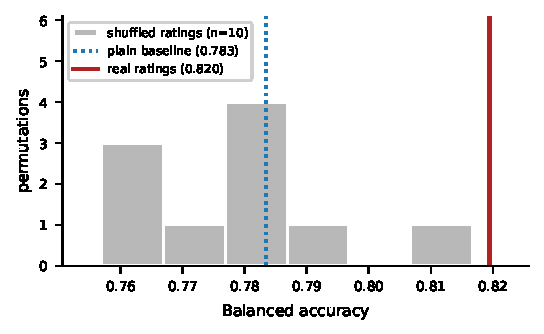
\includegraphics[width=\linewidth]{figures/permutation_hist_balanced_accuracy.pdf}
\caption{Permutation test for the quality signal. Grey: balanced accuracy when the lesion-to-rating assignment is permuted within each training fold, preserving the weight distribution exactly. Dotted: the plain baseline, which the null distribution is centred on. Solid: the real ratings, above every permutation drawn.}
\label{fig:perm}
\end{figure}

The control has also been informative negatively. The \emph{trust} variant's one apparent advantage, a narrower accuracy gap between the highest and lowest quality terciles (0.082 against the baseline's 0.091), narrows further still under shuffling, to 0.021, while its balanced accuracy falls from 0.788 to 0.763: a weighting carrying no quality information produces a flatter profile than the mechanism intended to produce one. That advantage is therefore reported as a reversed finding rather than a second positive result.

\subsection{Comparison with the Literature}
\label{sec:comparison}
This paper's channel-gated baseline, \emph{hard\_mining} variant, and best configuration have reached 0.783, 0.820 and 0.840 balanced accuracy respectively, against the closest published binary-task work. PAD-UFES-20's six-class balanced accuracies (0.765--0.842) are not valid comparators for a binary task despite the shared metric name. The binary result we have verified directly is Uliana and Krohling's \cite{diffmic}, 0.836 from a diffusion classifier over 2298 images under five-fold cross-validation, at the image level rather than our lesion level. This paper's best configuration has reached 0.840 $\pm$ 0.095. The nominal 0.004 difference is more than twenty times smaller than our own fold-to-fold standard deviation, so the two results are statistically indistinguishable and we have described ours as within noise of that benchmark rather than as exceeding it. The comparison is also not like for like: the two counts differ in unit, our 234 lesions against their 2298 images, and the underlying datasets differ by roughly sevenfold in lesion count and, more consequentially, in class balance, 17.9\% malignant here against 47.5\% there. HAM10000 \cite{ham10000} headline results have reached higher raw accuracy, but on a dermoscopy-only task with no metadata and roughly forty times more training images, and have not been treated as comparable.

MCR-SL has had no prior published benchmark, so this result is the current best on it by default; we have avoided framing that as a state-of-the-art claim, since there has been no prior number to surpass, and have emphasized the loss mechanism and its validation (Section~\ref{sec:main}) as the principal contribution.

\subsection{Ablation Study}
Eleven follow-up configurations have been evaluated. Sharpness-aware minimization with test-time augmentation has reached 0.822, the best of this sweep; focal loss has raised specificity to 0.923 while preprocessing gave the highest sensitivity, 0.736, trading off in opposite directions. Contrastive pretraining, the alternative optimizer, and quality-aware training have each underperformed the baseline, a convergent negative result across three independent interventions. Stacking every promising intervention together has underperformed both the baseline and its components, 0.759 against 0.783 and 0.822.

Applying the two evaluation-time interventions on top of \emph{hard\_mining}, rather than on top of the plain baseline, has produced this paper's best configuration. Table~\ref{tab:breakdown} decomposes it. Test-time augmentation has raised balanced accuracy to 0.833 and sensitivity to 0.808, the highest sensitivity of any configuration reported here; adding multi-image averaging has raised balanced accuracy further to 0.840 $\pm$ 0.095. Notably, multi-image averaging has stacked cleanly here, whereas it reduced balanced accuracy when combined with sharpness-aware minimization and test-time augmentation in the sweep above; that non-additivity has therefore been specific to that combination rather than a general property of the intervention.

The decomposition matters for how the headline number should be read. Of the total 0.057 gain over the baseline, 0.037, or roughly 65\%, has come from the quality-adaptive loss and has been causally validated in Section~\ref{sec:main}. The remaining 0.020 has come from generic evaluation-time averaging that requires no retraining and has nothing to do with image quality. We state this split explicitly so that the contribution attributable to the proposed mechanism is not overstated by the final figure.

\begin{table}[htbp]
\caption{Decomposition of the best configuration. Only the first step uses the quality signal; the remainder is generic evaluation-time averaging}
\label{tab:breakdown}
\centering
\scriptsize
\setlength{\tabcolsep}{3pt}
\begin{tabular}{|l|c|c|c|c|}
\hline
\textbf{Step} & \textbf{Quality?} & \textbf{Bal.\ acc.} & \textbf{$\Delta$} & \textbf{Sens.} \\
\hline
Channel-gated baseline & no & 0.783 & --- & 0.672 \\
$+$ \emph{hard\_mining} loss & \textbf{yes} & 0.820 & \textbf{$+$0.037} & 0.764 \\
$+$ test-time augmentation & no & 0.833 & $+$0.050 & \textbf{0.808} \\
$+$ multi-image averaging & no & \textbf{0.840} & $+$0.057 & 0.783 \\
\hline
\emph{hard\_mining}, shuffled & control & 0.775 & $-$0.008 & 0.667 \\
\hline
\end{tabular}
\end{table}

\subsection{Robustness Analyses}
\label{sec:robustness}
These analyses use the channel-gated out-of-fold predictions over the 231 lesions carrying both a prediction and a quality rating; three of the 234 lacked a usable image in their assigned test fold and were excluded rather than imputed.

\textbf{Quality-stratified performance.} Terciles by mean expert rating give accuracies of 0.776, 0.914 and 0.868 (low, mid, high; sizes 85, 93, 53, uneven because the mean of up to three integer ratings takes few distinct values). The pattern is not monotonic and Spearman correlation between rating and error is $-0.093$ ($p=0.158$): no strong quality-performance relationship is detected at 231 lesions, neither confirming nor ruling one out.

The validated \emph{hard\_mining} configuration has not flattened this profile: its high-minus-low accuracy gap has remained 0.091. Its benefit has appeared within terciles instead, most visibly on the lowest-quality one, where malignant sensitivity has risen from 0.667 to 0.810. The mechanism has improved detection on poor images without equalizing accuracy across quality levels, and we have not claimed the latter.

\textbf{Reversed findings.} Three apparently positive results have not survived scrutiny and are reported rather than omitted. \emph{Trust}'s narrower quality-tercile gap was undercut by the shuffled control narrowing it further (Section~\ref{sec:main}). A pooled correlation between expert certainty and prediction error, initially $\rho=-0.175$ ($p=0.008$, $N=231$), dissolved once stratified by class ($p=0.083$ and $p=0.559$), having reflected class composition rather than an independent relationship. And a proposed change to train on all images per lesion proved on verification to describe what the pipeline already did. At this sample size an uncontrolled first look repeatedly produces positives that controls dissolve, and reporting that pattern is part of the contribution.

\textbf{Intra-subject consistency.} Of 55 subjects with two or more evaluable lesions, 27 were perfectly consistent against a permutation null mean of 29.9 ($p=0.954$), and none had all lesions misclassified: errors have not concentrated in particular patients.

\textbf{Histopathology-confirmed versus panel-consensus.} The model has performed worse on the 28 histopathology-confirmed lesions than on the 203 panel-consensus-only ones, 0.750 against 0.867 accuracy, plausibly because histopathology is more often ordered for clinically ambiguous lesions. With 28 lesions this has been treated as qualitative only.



\subsection{Qualitative Analysis: Hard Samples}
\label{sec:qualitative}
Gradients have been taken with respect to the feature map \emph{after} the metadata gate, the representation the decision is computed from, with the metadata branch held fixed. Fig.~\ref{fig:hardsamples} compares the baseline and reweighted models on the two lowest-quality malignant lesions the loss has flipped from a miss to a correct call.

In (a), a basal cell carcinoma rated 5.7, the baseline has assigned $P=0.02$, a confident miss, with attention spread diffusely; under reweighting attention contracts onto a single focus and the call becomes $P=0.89$. In (b), a melanoma rated 4.3, baseline attention falls on the left edge away from the pigmented region and the lesion is missed at $P=0.27$; under reweighting attention moves onto the lesion and the call becomes $P=0.89$. Both lie in the lowest quality tercile, where reweighting assigns its largest weights.

These are illustrative rather than representative: across the 231 lesions the reweighting fixes six malignant lesions and breaks two, a net gain of four, which is what a $+0.092$ sensitivity amounts to at this scale.

\begin{figure}[htbp]
\centering
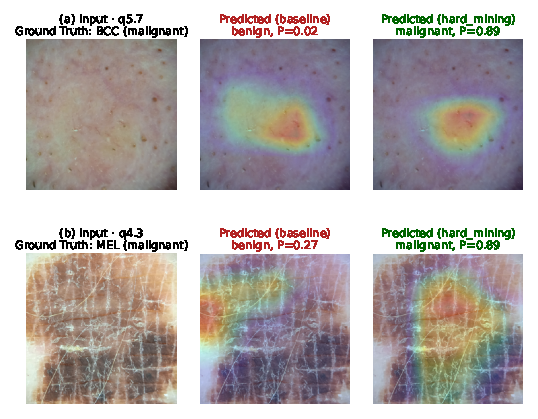
\includegraphics[width=\linewidth]{figures/hard_samples_gradcam_compare_1col.pdf}
\caption{Grad-CAM on the post-gate feature map for the two lowest-quality lesions that quality-adaptive reweighting has flipped from a miss to a correct call. Left column: \textbf{Input} (the diagnostic image), with expert quality rating $q$. Centre and right: \textbf{Prediction (baseline)} and \textbf{Prediction (\emph{hard\_mining})}, each with its $P(\mathrm{malignant})$ and outcome. \textbf{Ground Truth} is malignant for both: (a) basal cell carcinoma, (b) melanoma. Maps are $7\times7$ upsampled, indicating approximate attention only.}
\label{fig:hardsamples}
\end{figure}

\section{Conclusion and Future Work}
This paper has proposed quality-adaptive loss reweighting, scaling each training sample's classification loss by a real expert-assigned rating of its diagnostic image. Up-weighting low-quality samples has improved balanced accuracy by 0.037, sensitivity by 0.092 and AUROC by 0.025 over an identical baseline, and evaluation-time averaging on top has reached 0.840 $\pm$ 0.095; of that 0.057 total gain, 65\% is attributable to the loss and the remainder to generic technique. The validated direction is the opposite of the face recognition precedents that motivated it \cite{adaface,magface}, plausibly because a dermatologist can usually still diagnose from a degraded photograph while a degraded face can lose its identity entirely.

The effect size deserves care. A gain of 0.037 is comparable to the fold-to-fold standard deviation of roughly 0.08, and no paired fold-level test reaches significance at $N=5$. The claim rests instead on the permutation test: reweighting by permuted ratings returns performance to baseline, and the real result lies above every permutation drawn. We regard causal evidence as the appropriate standard at this scale, and have reported the effect size plainly rather than letting the final figure carry the claim. Two questions have been answered differently: performance shows no significant relationship with expert-rated quality, a null that also held for expert certainty once class composition was controlled, yet the objective has still exploited that signal.

The study is limited by MCR-SL's size, 234 usable lesions from one institution with 28 histopathology-confirmed, by a single training seed, and by a 17.9\% malignant rate leaving eight or nine malignant lesions per test fold. Future work should validate the mechanism on other quality-labelled medical datasets, most directly DeepDRiD \cite{deepdrid}, which records per-image quality alongside diabetic retinopathy grades and which we have prepared but not completed within this cycle, and should give numeric metadata fields representational capacity comparable to categorical embeddings.

\begin{thebibliography}{00}
\bibitem{mcrsl} M. Castro-Fernandez \emph{et al.}, ``MCR-SL: A multimodal, context-rich skin lesion dataset for skin cancer diagnosis,'' \emph{Data}, vol. 10, no. 10, art. 166, 2025.
\bibitem{esteva2017} A. Esteva, B. Kuprel, R. A. Novoa, J. Ko, S. M. Swetter, H. M. Blau, and S. Thrun, ``Dermatologist-level classification of skin cancer with deep neural networks,'' \emph{Nature}, vol. 542, pp. 115--118, 2017.
\bibitem{ham10000} P. Tschandl, C. Rosendahl, and H. Kittler, ``The HAM10000 dataset, a large collection of multi-source dermatoscopic images of common pigmented skin lesions,'' \emph{Sci. Data}, vol. 5, art. 180161, 2018.
\bibitem{metablock} A. G. C. Pacheco and R. A. Krohling, ``An attention-based mechanism to combine images and metadata in deep learning models applied to skin cancer classification,'' \emph{IEEE J. Biomed. Health Inform.}, vol. 25, no. 9, pp. 3554--3563, 2021.
\bibitem{paduf20} A. G. C. Pacheco \emph{et al.}, ``PAD-UFES-20: A skin lesion dataset composed of patient data and clinical images collected from smartphones,'' \emph{Data in Brief}, vol. 32, art. 106221, 2020.
\bibitem{se} J. Hu, L. Shen, and G. Sun, ``Squeeze-and-excitation networks,'' in \emph{Proc. IEEE Conf. Computer Vision and Pattern Recognition (CVPR)}, 2018.
\bibitem{efficientnet} M. Tan and Q. V. Le, ``EfficientNet: Rethinking model scaling for convolutional neural networks,'' in \emph{Proc. Int. Conf. Machine Learning (ICML)}, 2019, pp. 6105--6114.
\bibitem{imagenet} J. Deng, W. Dong, R. Socher, L.-J. Li, K. Li, and L. Fei-Fei, ``ImageNet: A large-scale hierarchical image database,'' in \emph{Proc. IEEE Conf. Computer Vision and Pattern Recognition (CVPR)}, 2009, pp. 248--255.
\bibitem{sam} P. Foret, A. Kleiner, H. Mobahi, and B. Neyshabur, ``Sharpness-aware minimization for efficiently improving generalization,'' in \emph{Proc. Int. Conf. Learning Representations (ICLR)}, 2021.
\bibitem{adamw} I. Loshchilov and F. Hutter, ``Decoupled weight decay regularization,'' in \emph{Proc. Int. Conf. Learning Representations (ICLR)}, 2019.
\bibitem{supcon} P. Khosla \emph{et al.}, ``Supervised contrastive learning,'' in \emph{Advances in Neural Information Processing Systems (NeurIPS)}, vol. 33, 2020, pp. 18661--18673.
\bibitem{focal} T.-Y. Lin, P. Goyal, R. Girshick, K. He, and P. Doll\'ar, ``Focal loss for dense object detection,'' in \emph{Proc. IEEE Int. Conf. Computer Vision (ICCV)}, 2017, pp. 2980--2988.
\bibitem{diffmic} J. J. M. Uliana and R. A. Krohling, ``Diffusion models applied to skin and oral cancer classification,'' 2025, arXiv:2504.00026. [Online]. Available: https://arxiv.org/abs/2504.00026
\bibitem{adaface} M. Kim, A. K. Jain, and X. Liu, ``AdaFace: Quality adaptive margin for face recognition,'' in \emph{Proc. IEEE/CVF Conf. Computer Vision and Pattern Recognition (CVPR)}, 2022.
\bibitem{magface} Q. Meng, S. Zhao, Z. Huang, and F. Zhou, ``MagFace: A universal representation for face recognition and quality assessment,'' in \emph{Proc. IEEE/CVF Conf. Computer Vision and Pattern Recognition (CVPR)}, 2021.
\bibitem{hu2023} M. Hu and X. Yang, ``Attention-driven lightweight model for pigmented skin lesion detection,'' 2023, arXiv:2308.02119. [Online]. Available: https://arxiv.org/abs/2308.02119
\bibitem{qgdr} Y. Pan, X. Cai, P. Xiong, F. Mei, Z. Wang, and J. Hong, ``From discarding to leveraging: quality-aware collaborative learning for robust diabetic retinopathy grading,'' \emph{Frontiers in Medicine}, vol. 13, art. 1795484, 2026.
\bibitem{deepdrid} R. Liu, X. Wang, Q. Wu \emph{et al.}, ``DeepDRiD: Diabetic retinopathy---grading and image quality estimation challenge,'' \emph{Patterns}, vol. 3, no. 6, art. 100512, 2022.
\end{thebibliography}

\end{document}
